\section{Results}\label{sec:results}

All results in this section use the main graph and the script-blocking status quo, unless stated
otherwise.

\subsection{RQ1: Does the origin of an outbreak matter?}\label{sec:rq1}
We use four origin groups, each disjoint from the others:
\begin{itemize}
  \item \emph{hubs}: the ten packages with the most direct dependents;
  \item \emph{bridges}: the ten with the highest betweenness among the remaining packages;
  \item \emph{mid-tier}: ten packages at the median k-core;
  \item \emph{leaves}: ten packages in the bottom 20\% by contagion out-degree.
\end{itemize}
We start 100 outbreaks from each package in each group, under four parameter scenarios
(\cref{tab:rq1,fig:rq1}).

\begin{table}[t]
\centering
\caption{RQ1: mean final outbreak size $\Rinf$ with 95\% bootstrap CI, and in parentheses the
probability of a major outbreak ($\Rinf\geq5\%$), by patient-zero group. Each cell aggregates 1{,}000 runs.}
\label{tab:rq1}
\small
\begin{tabular}{lcccc}
\toprule
Scenario & Hub & Bridge & Mid-tier & Leaf \\
\midrule
Spec reference & 5.3\% [5.1\%, 5.4\%] (46\%) & 0.8\% [0.8\%, 0.9\%] (0\%) & 0.2\% [0.2\%, 0.2\%] (0\%) & 0.0\% [0.0\%, 0.0\%] (0\%) \\
Dependency only & 2.6\% [2.5\%, 2.7\%] (11\%) & 0.2\% [0.2\%, 0.3\%] (0\%) & 0.0\% [0.0\%, 0.0\%] (0\%) & 0.0\% [0.0\%, 0.0\%] (0\%) \\
SH1-calibrated & 55.8\% [55.6\%, 55.9\%] (100\%) & 48.7\% [48.0\%, 49.4\%] (95\%) & 31.8\% [30.2\%, 33.3\%] (63\%) & 19.6\% [18.1\%, 21.0\%] (40\%) \\
SH2-calibrated & 85.8\% [85.7\%, 85.8\%] (100\%) & 84.2\% [83.4\%, 84.9\%] (98\%) & 78.8\% [77.2\%, 80.2\%] (92\%) & 55.4\% [52.8\%, 57.8\%] (64\%) \\
\bottomrule
\end{tabular}

\end{table}

\begin{figure}[t]
\centering
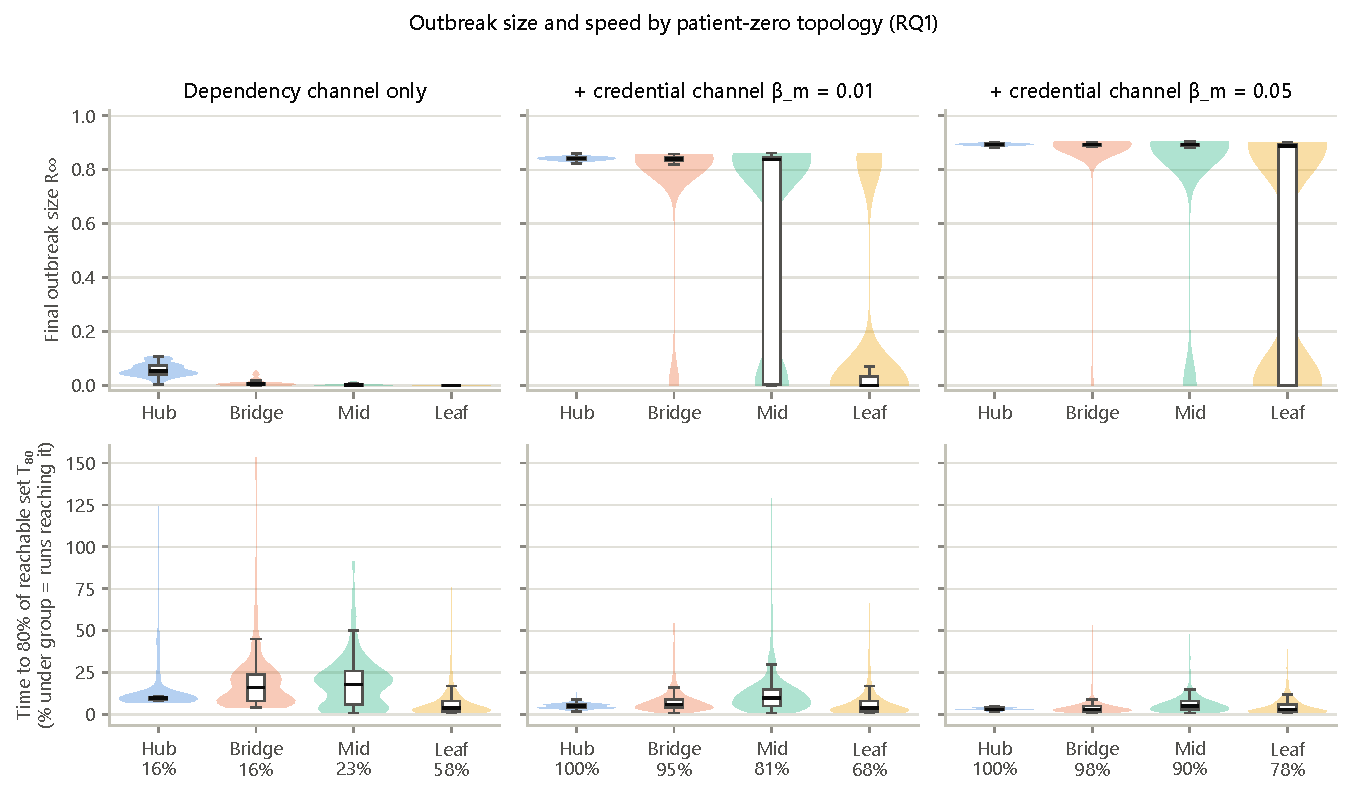
\includegraphics[width=\linewidth]{fig3_superspreader_comparison.pdf}
\caption{RQ1. Top: distributions of the final outbreak size $\Rinf$ by origin group and scenario. Bottom:
time to infect 80\% of the dependency-reachable set, for runs that reach it (the share of runs is shown
under each group).}
\label{fig:rq1}
\end{figure}

\paragraph{Dependency-only spread is bounded and hub-driven.}
In the spec-reference and dependency-only scenarios, outbreaks seeded at hubs reach \RQOneSpecRefHub{}
and \RQOneDepOnlyHub{} of the core, respectively. Outbreaks seeded at leaves essentially never spread.
Because the graph is nearly acyclic, an outbreak can only travel down the dependents of its origin, and
transmission is stochastic with $\beta<1$. A hub therefore reaches only a fraction of its static blast
radius before patching stops it. Topology matters strongly here, and the super-spreader hypothesis holds.

\paragraph{The credential channel erases most of the origin effect.}
With the SH1-calibrated credential channel:
\begin{itemize}
  \item hub-seeded outbreaks reach \RQOneShOneHub{} of the core;
  \item outbreaks seeded at leaves, which cannot spread at all through dependencies, still reach
        \RQOneShOneLeaf{} on average, with a major outbreak in \RQOneShOneLeafPmajor{} of runs.
\end{itemize}
Under SH2 parameters the corresponding figures are \RQOneShTwoHub{} and \RQOneShTwoLeaf. Between
\RQOneShOneLeafMaint{} and \RQOneShOneHubMaint{} of infections come through stolen tokens. Outbreak-size
distributions become strongly bimodal (\cref{fig:rq1}): an outbreak either dies out before a token leaks
or takes over most of the core. Origin topology mainly changes the \emph{probability} of take-off, not
the size of outbreaks that do take off. \Cref{fig:sir} shows the resulting epidemic curves.

\begin{figure}[t]
\centering
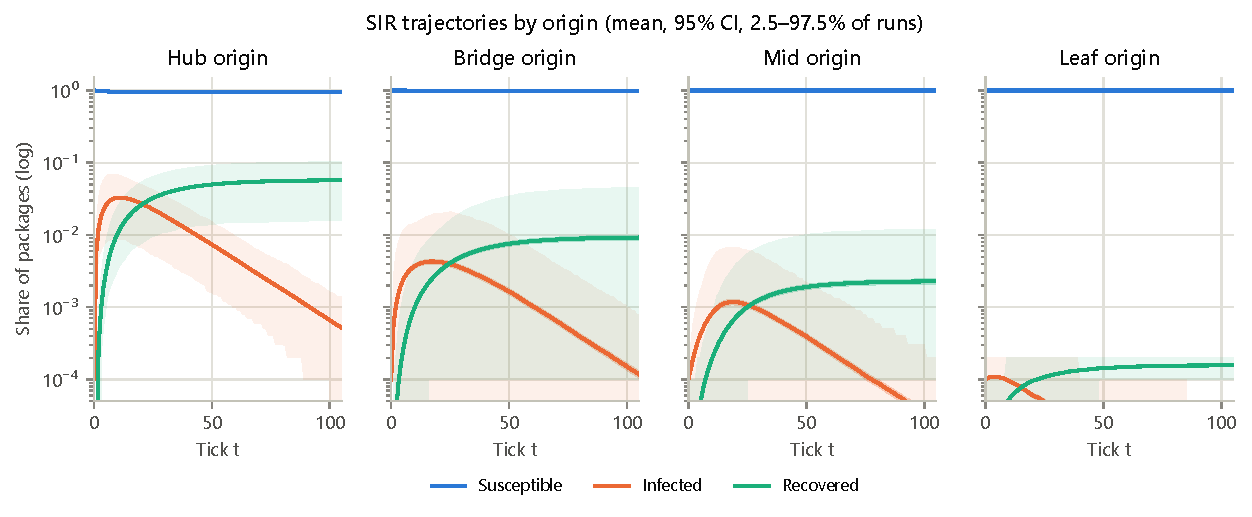
\includegraphics[width=\linewidth]{fig2_sir_epidemic_curves.pdf}
\caption{S/I/R trajectories (log scale) under SH1-calibrated parameters, by origin group: mean, 95\% CI
of the mean, and the 2.5--97.5\% envelope of runs. Patching starts at $t=24$\,h.}
\label{fig:sir}
\end{figure}

\subsection{RQ2: Which ecosystem regimes shift the threshold?}\label{sec:rq2}
We compare four regimes:
\begin{itemize}
  \item \emph{status quo}: the observed SemVer mix, with 10\% of packages blocking scripts;
  \item \emph{strict lockfile}: loose constraints pinned until 80\% of edges are exact;
  \item \emph{scripts disabled}: 70\% of packages block lifecycle scripts;
  \item \emph{hardened}: strict lockfiles, scripts disabled and trusted publishing on the top 5\% of hubs.
        In the hardened regime, stolen-token publishes to these hubs succeed with probability 0.1.
\end{itemize}
For each regime we sweep a 13$\times$5 grid of $(\beta,\gamma)$ with hub-seeded outbreaks and estimate
the critical $\beta_c$ at which the mean $\Rinf$ reaches 5\% (\cref{tab:rq2,fig:rq2}).

\begin{table}[t]
\centering
\caption{RQ2, dependency channel only ($\beta_m=0$): empirical critical transmission rate $\beta_c$ at
which mean $\Rinf$ reaches 5\%. ``none'' means that no grid value up to $\beta=1$ produced a major
outbreak.}
\label{tab:rq2}
\begin{tabular}{lccccc}
\toprule
Regime & $\gamma=0.02$ & $\gamma=0.05$ & $\gamma=0.10$ & $\gamma=0.20$ & $\gamma=0.40$ \\
\midrule
Status quo & 0.045 & 0.125 & 0.274 & 0.363 & 0.499 \\
Strict lockfile & 0.514 & 0.917 & none & none & none \\
Scripts disabled & 0.279 & 0.642 & none & none & none \\
Hardened & none & none & none & none & none \\
\bottomrule
\end{tabular}

\end{table}

\begin{figure}[t]
\centering
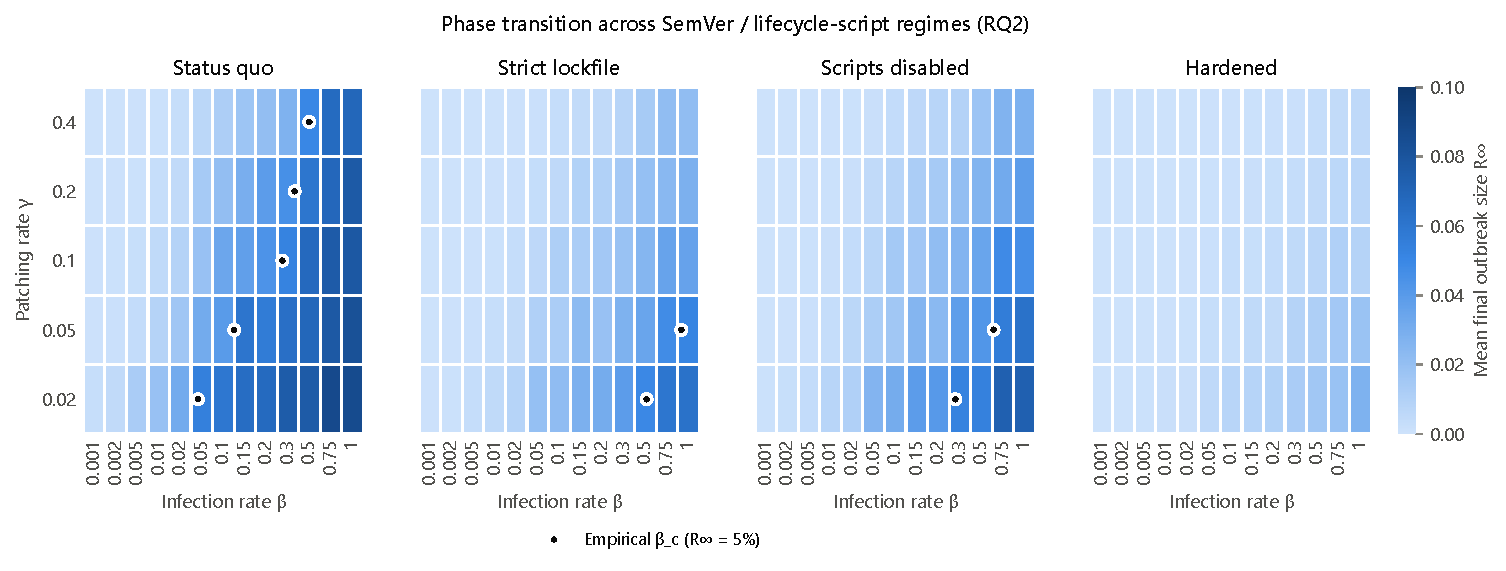
\includegraphics[width=\linewidth]{fig4_semver_phase_transition.pdf}
\caption{RQ2: mean $\Rinf$ over the $(\beta,\gamma)$ grid for each regime, dependency channel only.
Markers show the empirical $\beta_c$.}
\label{fig:rq2}
\end{figure}

\paragraph{Without stolen tokens, dependency-side hardening works.}
At $\gamma=\RQTwoGammaLow$ the status quo has $\beta_c=\RQTwoBetaSQ$. Strict lockfiles raise it to
\RQTwoBetaSL{} (about \RQTwoLockFactor$\times$), and blocking scripts on 70\% of packages raises it to
\RQTwoBetaSD{} (about \RQTwoScriptsFactor$\times$). The hardened regime never produces a major outbreak.
The spectral prediction $\tau_c=1/\lambda_{\max}=\RQTwoTauTheory$ lies far from these empirical
thresholds. This is expected for SIR on a nearly acyclic directed graph, where $1/\lambda_{\max}$ is only
a lower bound that is set by small monorepo cycles~\citep{li2013directed}.

\paragraph{With stolen tokens, the dependency threshold collapses.}
With the calibrated credential rates $\beta_m\in\{\CalOneBetaM,\CalTwoBetaM\}$, the estimated $\beta_c$
falls to the bottom of our grid (0.001) in \RQTwoCredCollapsed{} of regime--$\gamma$ combinations. The
credential channel alone sustains the epidemic, so the relevant threshold is in $\beta_m$, not $\beta$.
\Cref{tab:rq2b} reports the critical $\beta_m$ per regime at the SH1 transmission rate.
\RQTwoBDone

\begin{table}[t]
\centering
\caption{RQ2b: empirical critical token-leak rate $\beta_{m,c}$ per regime at $\beta=\CalOneBeta$.}
\label{tab:rq2b}
\begin{tabular}{lccccc}
\toprule
Regime & $\gamma=0.02$ & $\gamma=0.05$ & $\gamma=0.10$ & $\gamma=0.20$ & $\gamma=0.40$ \\
\midrule
Status quo & $\leq$0.001 & 0.001 & 0.002 & 0.008 & 0.020 \\
Strict lockfile & 0.001 & 0.002 & 0.005 & 0.015 & 0.031 \\
Scripts disabled & $\leq$0.001 & 0.001 & 0.004 & 0.012 & 0.028 \\
Hardened & 0.002 & 0.006 & 0.015 & 0.038 & 0.087 \\
\bottomrule
\end{tabular}

\end{table}

\subsection{RQ3: Patch reactively or immunize proactively?}\label{sec:rq3}
Outbreaks are seeded at hubs under SH1-calibrated parameters. Both reactive patching and natural
recovery begin only at the detection delay $t_{\text{det}}\in\{1,6,12,24,48\}$\,h.
\begin{itemize}
  \item Reactive policies treat up to $B$ packages per hour, either hubs first or at random.
  \item Proactive policies immunize $K$ packages at $t=0$, choosing them by betweenness, by degree or by
        acquaintance sampling.
\end{itemize}
To compare at equal cost, $K$ is set to the mean number of packages that hub patching treats at the same
$B$ and delay. \Cref{tab:rq3} reports paired reductions in $\Rinf$ at $B=\RQThreeBudget$ packages per hour
(\RQThreeBudgetPct{} of the graph), and \cref{fig:rq3} shows all budgets.

\begin{table}[t]
\centering
\caption{RQ3: share of the no-intervention outbreak prevented (paired, mean over 100 runs) at
$B=\RQThreeBudget$ per hour, by detection delay. The last row gives the no-intervention $\Rinf$, which
grows with the delay because natural patching also waits for detection.}
\label{tab:rq3}
\begin{tabular}{lccccc}
\toprule
Strategy & 1\,h & 6\,h & 12\,h & 24\,h & 48\,h \\
\midrule
Hub patching & 100\% & 90\% & 52\% & 13\% & 3\% \\
Random patching & 100\% & 76\% & 23\% & 5\% & 1\% \\
Firebreak (betweenness) & 3\% & 13\% & 27\% & 29\% & 26\% \\
Hub immunization & 6\% & 23\% & 38\% & 42\% & 40\% \\
Acquaintance & 3\% & 17\% & 32\% & 35\% & 34\% \\
\midrule
No intervention $R_\infty$ & 47\% & 48\% & 49\% & 55\% & 68\% \\
\bottomrule
\end{tabular}

\end{table}

\begin{figure}[t]
\centering
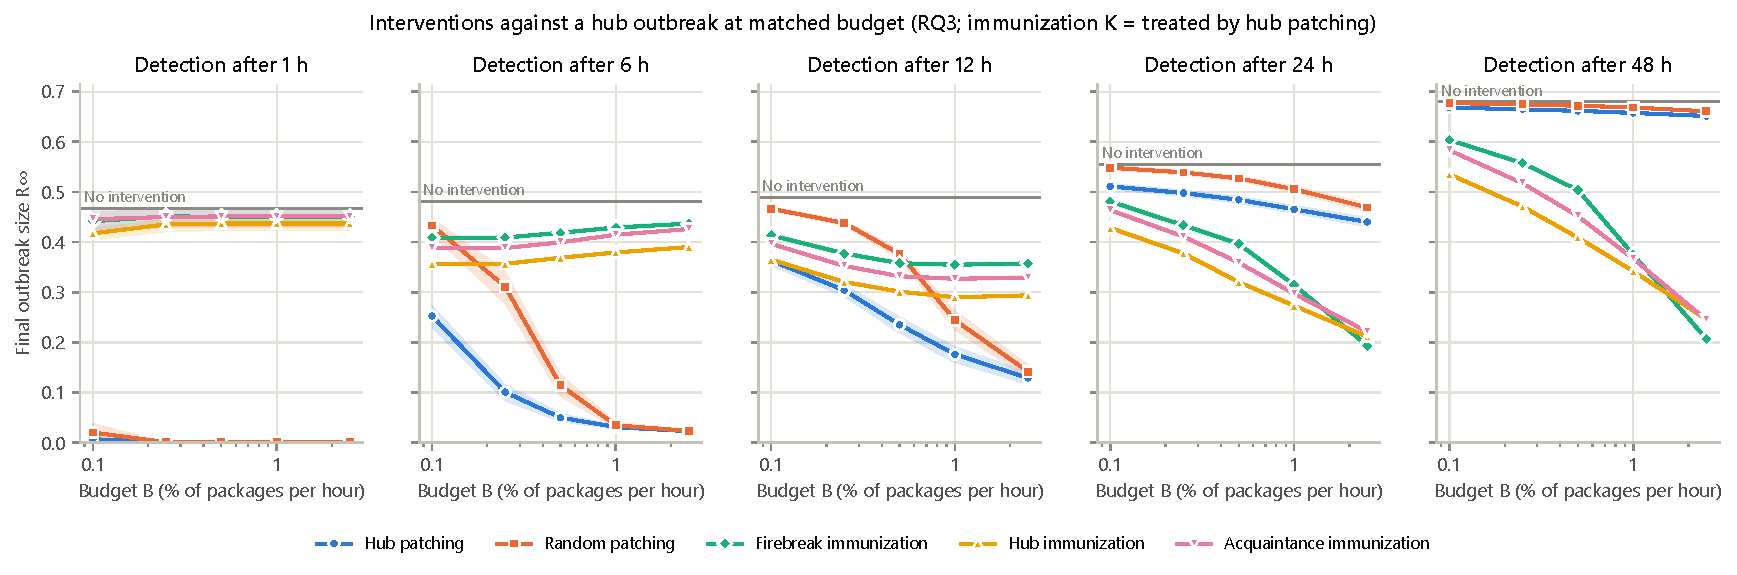
\includegraphics[width=\linewidth]{fig5_firebreak_immunization.pdf}
\caption{RQ3: final outbreak size against the intervention budget $B$ (95\% CI), by detection delay.
Proactive strategies immunize the same total number of packages that hub patching treats.}
\label{fig:rq3}
\end{figure}

\paragraph{Reactive patching works only with fast detection.}
Detected within an hour, the outbreak is almost fully contained by either reactive policy (hub patching
prevents \RQThreeHubPatchingOne). Its value drops quickly with delay: \RQThreeHubPatchingSix{} prevented
at 6\,h, \RQThreeHubPatchingTwelve{} at 12\,h, and only \RQThreeHubPatchingTwentyFour{} at 24\,h, which
was the lag of wave~1.

\paragraph{Proactive immunization holds up, and degree beats betweenness.}
Immunizing high-degree packages at the same total cost prevents \RQThreeHubImmunizationTwelve{} at 12\,h
and \RQThreeHubImmunizationTwentyFour{} at 24\,h. The two approaches cross over between 12 and 24\,h of
delay: reactive patching is still ahead at 12\,h, and proactive immunization is well ahead at 24\,h and
48\,h. Acquaintance immunization, which needs no global knowledge, comes close
(\RQThreeAcquaintanceTwentyFour{} at 24\,h).

Betweenness ``firebreaks'' are weaker under the credential channel (\RQThreeFirebreakBetweennessTwentyFour{}
at 24\,h). A plausible explanation is that betweenness targets packages that cut dependency paths,
whereas under the credential channel most infections bypass those paths through stolen tokens; we have
not tested this mechanism directly. Betweenness is a heuristic; optimized immunization sets could do
better~\citep{schneider2011limited}. Our claim is therefore limited to the comparison with degree-based
and random strategies at matched cost.
